\documentclass[10pt]{article}
\usepackage[T1]{fontenc}
\usepackage[margin=0.62in]{geometry}
\usepackage{array}
\usepackage{tikz}
\usetikzlibrary{arrows.meta,positioning,calc}

\pagestyle{plain}
\setlength{\parindent}{0pt}
\setlength{\parskip}{0.28em}
\emergencystretch=3em
\renewcommand{\arraystretch}{1.08}

\newcolumntype{L}[1]{>{\raggedright\arraybackslash}p{#1}}
\tikzset{
  box/.style={draw, rounded corners=1pt, align=center, inner sep=4pt, minimum height=8mm},
  edge/.style={-{Stealth[length=2mm]}, thick},
  faintedge/.style={-{Stealth[length=2mm]}, thick, dashed}
}

\begin{document}

\begin{center}
{\Large Hero Pill Dispenser --- UART Access \& Soldering}\\
{\normalsize Dense hardware-interface state model and gear/proof matrices}\\
Xiamen Zayata M115/M111 (FCC 2AN4DM115 / 2AN4DM111) --- worlds World U, 2026-06-02
\end{center}

\section*{Verdict}

\begin{center}\small
\begin{tabular}{|L{1.0in}|L{4.5in}|L{0.6in}|}
\hline
\textbf{Plane} & \textbf{Dense status} & \textbf{Gate} \\
\hline
Identity & Hero Smart Pill Dispenser; primary MCU TI CC3220 (Cortex-M4, SimpleLink) on M115/M111, ESP32 on sibling variants. UART debug pads bridge the hardware plane to the firmware/console plane. & fixed \\
\hline
Goal & Solder a 3-wire (TX/RX/GND) tap to the unpopulated UART header to gain logs, the \texttt{hero>} shell, and a firmware-extraction vector. & access \\
\hline
Hard rule & Dispenser is mains-powered by its own AC adapter: never wire VCC to the serial adapter (back-feed damages MCU/adapter). Only TX, RX, GND. & safety \\
\hline
Success claim & A valid tap requires correct pad ID, 3 clean joints, strain relief, 3.3\,V null-modem wiring, 115200-8N1 link, and a responding \texttt{hero>} prompt. & proof \\
\hline
\end{tabular}
\end{center}

\section{UART tap flow}

\begin{center}
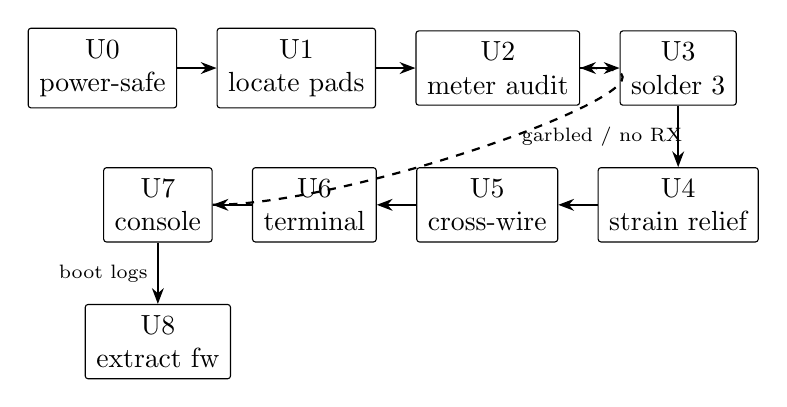
\begin{tikzpicture}[node distance=0.78cm and 0.5cm]
\node[box] (u0) {U0\\power-safe};
\node[box, right=of u0] (u1) {U1\\locate pads};
\node[box, right=of u1] (u2) {U2\\meter audit};
\node[box, right=of u2] (u3) {U3\\solder 3};
\node[box, below=of u3] (u4) {U4\\strain relief};
\node[box, left=of u4] (u5) {U5\\cross-wire};
\node[box, left=of u5] (u6) {U6\\terminal};
\node[box, left=of u6] (u7) {U7\\console};
\node[box, below=of u7] (u8) {U8\\extract fw};

\draw[edge] (u0) -- (u1);
\draw[edge] (u1) -- (u2);
\draw[edge] (u2) -- (u3);
\draw[edge] (u3) -- (u4);
\draw[edge] (u4) -- (u5);
\draw[edge] (u5) -- (u6);
\draw[edge] (u6) -- (u7);
\draw[edge] (u7) -- node[left, font=\scriptsize]{boot logs} (u8);
\draw[faintedge] (u7.east) to[out=0,in=0] node[right, font=\scriptsize]{garbled / no RX} (u2.east);
\end{tikzpicture}
\end{center}

\section{Tap state matrix}

\begin{center}\scriptsize
\begin{tabular}{|L{0.32in}|L{0.95in}|L{1.9in}|L{1.5in}|L{1.25in}|}
\hline
\textbf{S} & \textbf{Where} & \textbf{What / how} & \textbf{Why} & \textbf{Exit proof} \\
\hline
U0 & enclosure & Unplug AC, wait 60\,s, open base, secure PCB, wear grounded ESD strap. & Mains back-feed and ESD both kill the board before any proof. & De-energized, fixed, grounded. \\
\hline
U1 & near MCU & Find the unpopulated 4-pad header (\texttt{J1}/\texttt{TP1}/\texttt{UART0}): VCC, TX, RX, GND. & This header is the only hardware boundary into the console. & 4 pads identified. \\
\hline
U2 & meter audit & Continuity to shield/USB shell $\rightarrow$ GND; stable 3.3\,V $\rightarrow$ VCC; 3.3\,V that dips to 2.8--3.0\,V on boot $\rightarrow$ TX; solid pulled-up 3.3\,V $\rightarrow$ RX. & Pads are usually unlabeled; wrong guess back-feeds VCC. & All four roles mapped. \\
\hline
U3 & solder & Flux TX/RX/GND only; tin 30\,AWG Kynar; reflow onto pads. Leave VCC unconnected. & Three signals suffice; VCC is forbidden. & 3 clean joints, VCC NC. \\
\hline
U4 & strain relief & Kapton tape or hot-melt over joints; land wires on a 3-pin header strip. & Bare pads tear off on reassembly pull. & Joints mechanically anchored. \\
\hline
U5 & cross-wire & PCB TX$\rightarrow$adapter RX, PCB RX$\rightarrow$adapter TX, GND$\rightarrow$GND; adapter jumper at 3.3\,V. & Null-modem crossover plus 3.3\,V logic level. & 3.3\,V mode verified. \\
\hline
U6 & host link & 115200-8N1, no flow control; \texttt{screen}/\texttt{picocom}/\texttt{tio} on \texttt{/dev/cu.usbserial-*} or \texttt{/dev/ttyUSB*}. & Link config must match the MCU UART. & Port opens, no errors. \\
\hline
U7 & console & Power on; boot logs scroll; press Enter for \texttt{hero>}: \texttt{status}, \texttt{dispense}, \texttt{calibrate}, \texttt{diag}, \texttt{set}, \texttt{factory-reset}. & Only here is the interactive plane reached. & Prompt echoes a command. \\
\hline
U8 & extraction & CC3220: SimpleLink UART $\rightarrow$ TI UniFlash $\rightarrow$ read SLFS \texttt{mcuimg.bin} (non-secure R). ESP32: \texttt{esptool.py} read\_flash. & Firmware dump for static RE. & Plaintext image off-device. \\
\hline
\end{tabular}
\end{center}

\section{Access gained}

\begin{center}\scriptsize
\begin{tabular}{|L{1.4in}|L{4.6in}|}
\hline
\textbf{Capability} & \textbf{Detail} \\
\hline
Live system logs & FreeRTOS task spawn/schedule, WiFi RSSI/DHCP, MQTT client-id/keepalive/topics, TLS cipher/endpoints (\texttt{cloud.herohealth.com}, \texttt{id.herohealth.com}), stepper/home-sensor/vacuum telemetry. \\
\hline
\texttt{hero>} shell & \texttt{status} (heap/temp/batt/net/slots), \texttt{dispense <slot>}, \texttt{calibrate [slot]}, \texttt{diag} (raw sensor dump), \texttt{set <key> <value>} (WiFi/timezone), \texttt{factory-reset} (NVS erase). Med names hashed via \texttt{scramble\_med\_name} before serial TX. \\
\hline
Bootloader / extraction & CC3220 SimpleLink UART programming $\rightarrow$ UniFlash SLFS access $\rightarrow$ \texttt{mcuimg.bin}; ESP32 ROM loader $\rightarrow$ \texttt{esptool.py}. \\
\hline
Local provisioning & Read/write WiFi credentials and timezone directly via \texttt{set}, bypassing the cloud onboarding flow. \\
\hline
\end{tabular}
\end{center}

\section{Gear needed}

\begin{center}\scriptsize
\begin{tabular}{|L{1.05in}|L{4.95in}|}
\hline
\textbf{Class} & \textbf{Items} \\
\hline
Soldering & Fine-tip temperature-controlled iron, thin solder, flux pen/paste, 30\,AWG Kynar wire, 3-pin male + female-to-female Dupont headers. \\
\hline
Interface & 3.3\,V-capable USB-to-UART adapter (CP2102 / CH340 / FTDI) with selectable 3.3\,V level. \\
\hline
Bench & Multimeter (continuity + DC volts), Kapton tape / hot-melt for strain relief, plastic spudger + PH\#1 driver, ESD strap and mat. \\
\hline
Software & Terminal: \texttt{screen} / \texttt{picocom} / \texttt{tio} / \texttt{minicom} (PuTTY / Tera Term on Windows) at 115200-8N1. Dump: \texttt{esptool.py} (ESP32) or TI UniFlash (CC3220). \\
\hline
\end{tabular}
\end{center}

\section{Cross-wiring (null-modem, 3.3\,V)}

\begin{center}\scriptsize
\begin{tabular}{|L{1.3in}|L{1.6in}|L{3.1in}|}
\hline
\textbf{Hero PCB pad} & \textbf{Adapter pin} & \textbf{Note} \\
\hline
TX & RX & Dispenser transmit into adapter receive. \\
\hline
RX & TX & Adapter transmit into dispenser receive. \\
\hline
GND & GND & Common reference; required for any signal. \\
\hline
VCC & --- (NC) & Do not connect. Board is AC-powered; back-feed damages MCU/adapter. \\
\hline
\end{tabular}
\end{center}

\section{Troubleshooting}

\begin{center}\scriptsize
\begin{tabular}{|L{1.5in}|L{2.0in}|L{2.4in}|}
\hline
\textbf{Symptom} & \textbf{Likely cause} & \textbf{Fix} \\
\hline
Garbled text / symbols & Wrong baud or shifted MCU clock. & Force 115200-8N1; on ESP32 confirm 40 vs 26\,MHz crystal hasn't skewed the baud divisor. \\
\hline
TX visible, RX dead & Level mismatch, cold RX joint, or RX/TX crossed. & Adapter TX $\rightarrow$ PCB RX; set adapter to 3.3\,V (not 5\,V); reflow the RX joint. \\
\hline
No output at all & Missing common GND, crossed lines, or target held in reset. & Secure GND; swap RX/TX at adapter; TX should rest at 3.3\,V. \\
\hline
Boot-loops on connect & Adapter DTR/RTS pulling a strap pin (e.g. GPIO12) high. & Leave DTR/RTS disconnected; do not drive bootstrap pins during power-up. \\
\hline
\end{tabular}
\end{center}

\section{Evidence and artifacts}

\begin{itemize}
\item \texttt{u/hero\_uart\_soldering.md}: source procedure this PDF renders.
\item \texttt{a/hero\_fcc\_regulatory.md}: FCC ID 2AN4DM115 / 2AN4DM111, RF and MCU evidence.
\item \texttt{u/hero\_serial\_console.rs}: \texttt{hero>} command set and \texttt{scramble\_med\_name} hashing.
\item \texttt{f/hero\_flash\_extraction.md}: physical access and flash-dump path.
\item \texttt{i/hero\_jtag\_debug.md}: JTAG/SWD fallback when UART extraction is locked.
\item \texttt{b/hero\_firmware}: extracted firmware working set.
\end{itemize}

\textbf{Safety / scope.} Medical dispensing device. Tap only TX/RX/GND, never VCC. Authorized reverse engineering of owned hardware only; patient-identifying data is hashed before it crosses the serial line.

\end{document}
